% Name: Troubleshooting flowchart
% Description: Yes and no questions that lead to an action, laid out top to bottom.
% Tags: flowchart, decision, troubleshooting

\usetikzlibrary{shapes.geometric, arrows.meta, positioning}

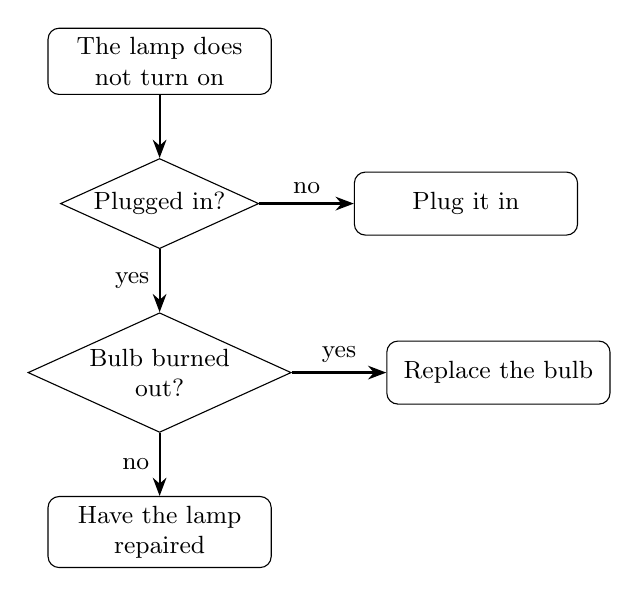
\begin{tikzpicture}[
  node distance=8mm and 12mm,
  every node/.style={font=\small, align=center},
  decision/.style={diamond, aspect=2.2, draw, inner sep=1pt},
  action/.style={rectangle, rounded corners, draw, minimum height=8mm, text width=26mm},
  arrow/.style={-{Stealth}, thick},
]
  \node[action] (start) {The lamp does\\not turn on};
  \node[decision, below=of start] (plug) {Plugged in?};
  \node[action, right=of plug] (fix1) {Plug it in};
  \node[decision, below=of plug] (bulb) {Bulb burned\\out?};
  \node[action, right=of bulb] (fix2) {Replace the bulb};
  \node[action, below=of bulb] (fix3) {Have the lamp\\repaired};

  \draw[arrow] (start) -- (plug);
  \draw[arrow] (plug) -- node[above] {no} (fix1);
  \draw[arrow] (plug) -- node[left] {yes} (bulb);
  \draw[arrow] (bulb) -- node[above] {yes} (fix2);
  \draw[arrow] (bulb) -- node[left] {no} (fix3);
\end{tikzpicture}
